\chapter{Lec 07 - Neural Networks I}

\section{Neural Networks}
An artificial neuron is a unit that computes a non-linear function over the inputs. Its output depends on the input and on the set of \textbf{weights}. These weights have to be learned.\newline\newline
An \textbf{Artificial Neural Network} is a system consisting of interconnected units that compute nonlinear (numerical) functions. Adjustable weights are associated with connections among units.\newline\newline
Deep Feed Forward Neural Networks, also called multi-layer perceptrons (MLP), approximate a function $f^{*}$ that maps an input $x$ to a category $y$. The MLP defines a mapping $\hat{y} = f(x;\theta)$ where $\theta$ is the set of parameters. They are typically represented as a composition of many different functions $f(x) = f^{(3)}(f^{(2)}(f^{(1)}(x)))$. The intermediate layers are called \textbf{hidden layers}, while the final layer is called \textbf{output layer}.\newline\newline
Multiple layers of cascaded units makes a Neural Network able to implement complex non linear functions. The non linearity of the model is given by the activation functions. In fact, without them (linear activation) the result of the model, even if it’s very complex, would still be linear.\newline\newline
\textbf{Example:}\newline
Let's try to define a linear model that predicts the XOR function.
\[Tr = \{ ([0,0], 0), ([0, 1], 1), ([1,0],1), ([1,1], 0)\} \quad f(\textbf{x};\textbf{w};b) = \textbf{x}\textbf{w}^{T} + b\]
The XOR function \textbf{cannot} be learned by any linear classifier. In order to solve this problem, we can define a two-layers Neural Network with the addition of the ReLU activation function $ReLU(y) = max(0, y)$. The networks becomes:
\[f(\textbf{x}; \textbf{W}, \textbf{c}, \textbf{w}, b) = \textbf{w}^{T} \, max(0, \textbf{W}\textbf{x}^{T} + \textbf{c}) + b\]
the following parameters values provide a solution to the XOR problem:
\[
    \textbf{W} =
    \begin{bmatrix}
        1 & 1\\
        1 & 1
    \end{bmatrix},
    \,\,
    \textbf{c} = 
    \begin{bmatrix}
        0 \\
        -1
    \end{bmatrix},
    \,\,
    \textbf{w} = 
    \begin{bmatrix}
        1 \\
        -2
    \end{bmatrix},
    \,\,
    b = 0
\]
Note that the first hidden layer has two nodes.\newline\newline
The most common activation functions are the following:
\begin{center}
    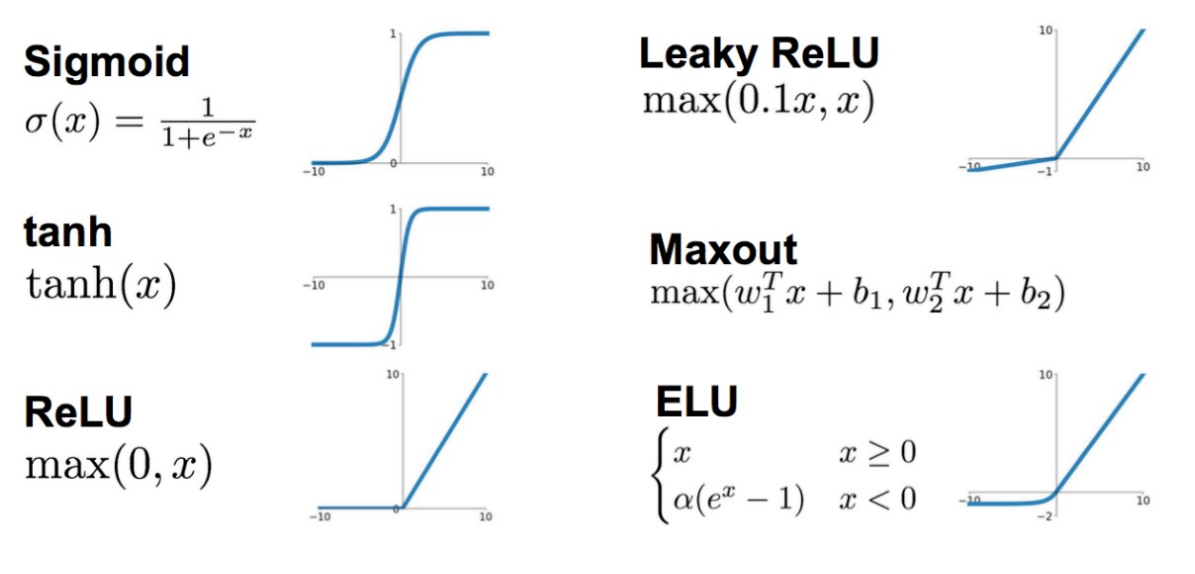
\includegraphics[scale = 0.6]{images/Activation Functions.png}
\end{center}
In general, the goal is to have a more complex decision surface. We can achieve this goal by using non-linear activation functions and stacking several hidden layers. In the XOR example above, the initial points are mapped by the first hidden layer into a new space where they are linearly separable. Thanks to this, the output linear layer is able to classify the points correctly.

\section{Learning in a Neural Network}
In general, the problem of how to update the weights of a model in order to minimize the committed error is called \textbf{credit assignment problem}. A possible solution is to make a single neuron \textbf{derivable} and exploit gradient descent technique to learn the \textit{right} weights. In order to make a neuron derivable, its activation function must be derivable.\newline\newline
Linear models (e.g. SVM) are formulated as \textbf{convex models}. However, the non-linearity in neural networks makes the problem \textbf{non-convex}. It means that there is no guarantee of achieving the global optimum. Furthermore, the way in which the weight of a NN are initialized has a strong impact on the solution that the model will find.

\section{Cost Function}
A important aspect of the design of a deep neural network is the choice of the cost function. In most cases, the model defines a distribution $p(\textbf{y} | \textbf{x}; \theta)$ and the cost function is the cross-entropy between training labels and network predictions (negative log-likelihood):
\[J(\theta) = - E_{(x,y) \sim \hat{p}_{data}}log\, p_{model}(\textbf{y}|\textbf{x})\]
The specific form of the cost function changes from model to model. The output representation $\textbf{h} = f(\textbf{x};\theta)$ determines the form of the cross-entropy function.
\begin{itemize}
    \item \textbf{Linear Regression:} If we assume that the target values are distributed according to a Gaussian distribution $G$, we can think our output layer as to produce the mean of $G$.
    \[\hat{\textbf{y}} = \textbf{W}^{T}\textbf{h} + \textbf{b}\]
    \[G(\textbf{y};\hat{\textbf{y}}; \textbf{I})\]
    As we already seen, in this case maximizing the likelihood corresponds to minimize the mean squared error.
    \[J(\theta) = \frac{1}{2}E_{p \sim \hat{p}_{data}}(y - f(\textbf{x}; \theta))^{2} + constant\]
    Basically, this is a motivation of why the mean squared error cost function is suitable for linear regression.

    \item \textbf{Binary classification:} In this case we assume that our targets are distributed according to a Bernoulli distribution. This distribution depends on a single parameter $\phi \in [0, 1]$:
    \begin{itemize}
        \item $P(\text{x} = 1) = \phi$
        \item $P(\text{x} = 0) = 1 - \phi$
    \end{itemize}
    In general:
    \[P(\text{x} = x) = \phi^{x}(1 - \phi)^{1-x}\]
    The NN just needs to predict $P(\text{y} = 1 | \textbf{x})$. Therefore, we want to force this number to lie in $[0, 1]$. For example, we can use the following function:
    \[P(\text{y} = 1|\textbf{x}) = max(0, min(1, \textbf{w}^{T}\textbf{h} + b))\]
    However, this is not a good choice for gradient descent. In fact, if the output is outside $[0, 1]$ the function is not derivable and the gradient will always be 0. We want to ensure that there is always some gradient when the model is wrong. An alternative way to force the output to lie in $[0, 1]$ is to use an \textbf{output} linear layer with a \textbf{sigmoid activation function}.
    \[\hat{y} = \sigma(\textbf{w}^{T}\textbf{h} + b)\]
    where $\sigma$ is a Sigmoid or Logistic function:
    \[\sigma(x) = \frac{1}{1 + e^{-x}}\]
    \begin{center}
        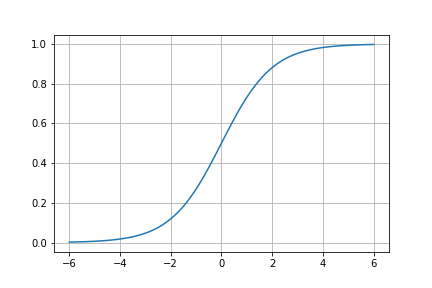
\includegraphics[scale = 0.5]{images/sigmoid.png}
    \end{center}
    An output unit is composed of two components:
    \begin{itemize}
        \item $z = \textbf{w}^{T}\textbf{h} + b$
        \item $\sigma(\cdot)$: the activation function to \textbf{convert $z$ into a probability} (in order to apply maximum likelihood optimization).
    \end{itemize}
    How can we define a probability distribution over $y$ using the value $z$ ? The sigmoid can be motivated by constructing an unnormalized probability distribution $\hat{P}(y)$, which does not sum to 1. We assume that the unnormalized probabilities are linear in $y$ and $z$.
    \[log\, \hat{P}(y) = yz \quad i.e. \,\, log\, \hat{P}(y = 1) = z, \,\, log\, \hat{P}(y = 0) = 0\]
    We can exponentiate to obtain the unnormalized probabilities:
    \[\hat{P}(y) = e^{yz}\]
    Then, we normalize to obtain a proper probablity:
    \[P(y) = \frac{e^{yz}}{\sum_{y'=0}^{1} e^{y'z}} = \sigma((2y - 1)z)\]
    where:
    \begin{itemize}
        \item $P(y = 1) = \frac{1}{1 + e^{-z}}$
        \item $P(y = 0) = \frac{1}{1 + e^{z}}$
    \end{itemize}
    As we already seen, the cost function used with maximum likelihood is the negative-log likelihood. Therefore, the loss function for maximum likelihood learning of a Bernoulli parametrized by a sigmoid is:
    \[J(\theta) = -log\, P(y|\textbf{x}) = -log\,\sigma((2y - 1)z) = \zeta((1 - 2y)z)\]
    where $\zeta(x) = log(1 - exp(x))$ is called \textbf{softplus} function.\newline\newline
    This approach to predicting the probabilities in log-space is natural to use with maximum likelihood learning. The log in the cost function undoes the exp of the sigmoid. Without this effect, the saturation of the sigmoid could prevent gradient- based learning from making good progress.\newline\newline
    The saturation (i.e. when the gradient is very small) occurs when $y = 1$ and $z$ is very positive or $y = 0$ and $z$ is very negative, that is, when the model has the right answer.\newline\newline
    With other cost functions, such as MSE, we'll be able to find a solution but it would \textbf{not} be the maximum-likelihood solution.

    \item \textbf{Multi-class classification:} In this case the output has to be a probability distribution over a discrete variable with $n$ possible values. We have to generate a vector $\hat{\textbf{y}}= [\hat{y}_0, \hat{y}_1, ..., \hat{y}_{n-1}]$ where:
    \begin{itemize}
        \item $\hat{y}_i = P(y = i | \textbf{x})$
        \item $\forall i,\,\, 0 \leq \hat{y}_i \leq 1$
        \item $\sum_i \hat{y}_i = 1$
    \end{itemize}
    We can use the same approach for the Bernoulli distribution generalized to the \textbf{Multinoulli distribution}:
    \[\textbf{z} = \textbf{W}^{T}\textbf{h} + \textbf{b} \quad \text{where}\,\, z_i = log\, \hat{P}(y = i | x)\]
    In order to represent the probability distribution over $n$ different classes, we can use the \textbf{Softmax} function, which is a generalization of sigmoid.
    \[softmax(\textbf{z})_i = \frac{e^{z_i}}{\sum_j^n e^{z_j}}\]
    By applying the log-likelihood, the cost function is:
    \[log\, softmax(\textbf{z})_i = z_i - log \, \sum_j e^{z_j}\]
    $z_i$ pushes the correct labels up and $log \, \sum_j e^{z_j}$ pushes the uncorrect labels down. When we perform the prediction, we'll choose the argmax of $\hat{\textbf{y}}$.
\end{itemize}

\subsection{Output functions in general}
Linear, sigmoid and softmax output units are the most common, but NN can generalize to almost any kind of output layer.\newline\newline
Maximum likelihood provides a guide to design almost any output layer.
\begin{enumerate}
    \item We define a conditional distribution $p(\textbf{y}|\textbf{x}; \theta)$
    \item As cost function, maximum likelihood suggest to use $-log\, p(\textbf{y}|\textbf{x}; \theta)$
\end{enumerate}
We can think of the NN as $f(\textbf{x}; \theta) = \omega$ where $\omega$ are the parameters of a distribution over $\textbf{y}$ and the cost function is $-log\, p(\textbf{y};\omega(\textbf{x}))$

\section{Hidden units}
An hidden unit can be described as accepting an input $x$, computing $z = W^{T}x + b$, and applying an element-wise nonlinear function $g(z)$. The design of hidden units does not have many definitive guiding theoretical principle. What we can do is to evaluate hidden units performance on a validation set. To select the most suitable activation function we can rely on some basic intuitions motivating each type of hidden unit.

\subsection{Hidden units: ReLU}
An hidden unit with ReLU activation function is defined as follows:
\[g(z) = max(0, z) \quad z = f(\textbf{W}^{T}\textbf{x} + \textbf{b})\]
Such hidden units are similar to linear units and therefore easier to optimize. However, ReLU units do not learn via gradient-based methods on examples for which their activation is zero. In order to solve this problem, generalizations of ReLU have been defined (e.g. leakyReLU) $g(z, \alpha)_i = max(0, z_i) + \alpha_i \, min(0, z_i)$.

\subsection{Hidden units: Tanh and sigmoid}
Other common activation functions are Tanh and sigmoid:
\begin{itemize}
    \item Logistic sigmoid: $g(z) = \sigma(z)$
    \item Hyperbolic Tangent: $g(z) = tanh(z) = 2\sigma(2z) - 1$
\end{itemize}
Actually, these two functions are not a very good choice for the hidden layers since they saturate across most of their domain. In particular, they saturate to high value when $z$ is very positive, and to low value when $z$ is very negative. This is good for output units, as we seen before, but not for hidden units, because in hidden layers we just want to keep learning without necessarily having a value between 0 and 1. Tanh typically performs better than the logistic sigmoid.\newline\newline
In general, many differentiable functions are reasonable (e.g. $cos(x)$), but they show no significant advantage over common ones.

\section{Architecture}
The architecture of a NN is its overall structure. Neural networks are generally organised in layers where each layer is a function of the preceding one:
\[\textbf{h}^{(1)} = g^{(1)}(\textbf{W}^{(1)T}\textbf{x} + \textbf{b}^{(1)})\]
\[\textbf{h}^{(i)} = g^{(i)}(\textbf{W}^{(i)T}\textbf{h}^{(i - 1)} + \textbf{b}^{(i)})\]
The main architectural considerations are:
\begin{itemize}
    \item The depth of the network
    \item The width of each layer
\end{itemize}
Deeper networks tend to generalize better, but they are harder to train.\newline\newline
All these hyper-parameters should be validated on a validation set.\newline\newline
\textbf{Universal approximation Theorem}\newline\newline
Given a feed-forward NN with just one hiddel layer, any continuous function $f:\mathbb{R}^{n} \rightarrow \mathbb{R}$ and an arbitrarily small $\epsilon > 0$, then, for a large class of activation functions, there always exists an integer $M$ such that the function $g: \mathbb{R}^{n} \rightarrow \mathbb{R}$ computed by the net using at least $M$ hidden units approximates the function $f$ with tolerance $\epsilon$, that is:
\[max_{x \in \Omega}|f(\textbf{x}) - g(\textbf{x})| < \epsilon\]
Note that the theorem attests the existence of a NN with $M$ hidden units that approximates any continuous function with the desired tolerance, but it says nothing about how $M$ can be computed and how large this network would be. Furthermore, we are not guaranteed that the training algorithm will be able to learn it (the optimization algorithm may not be able to find the value of the parameters that corresponds to the desired function).\newline\newline
Using deeper models can reduce the number of units required to represent the desired function. Furthermore, greater depth does seem to result (empirically) in better generalization for a wide variety of tasks.\newline\newline
Many neural networks architectures have been developed for specific tasks, e.g. Convolutional Neural Networks (CNN) or Recurrent Neural Network (RNN). In general, the layers need to be connected in a chain:
\begin{itemize}
    \item Skip connections: Make it easier for the gradient to flow from output layers to layers nearer the input.

    \item Sparse connections: Each unit in a layer is connected to only a small subset of units in the next layer.
\end{itemize}
